\section{Resultado final}

El resultado final de la animación es el siguiente:


\begin{figure}[H]
    \centering
    \begin{subfigure}[t]{0.48\textwidth}
        \centering
        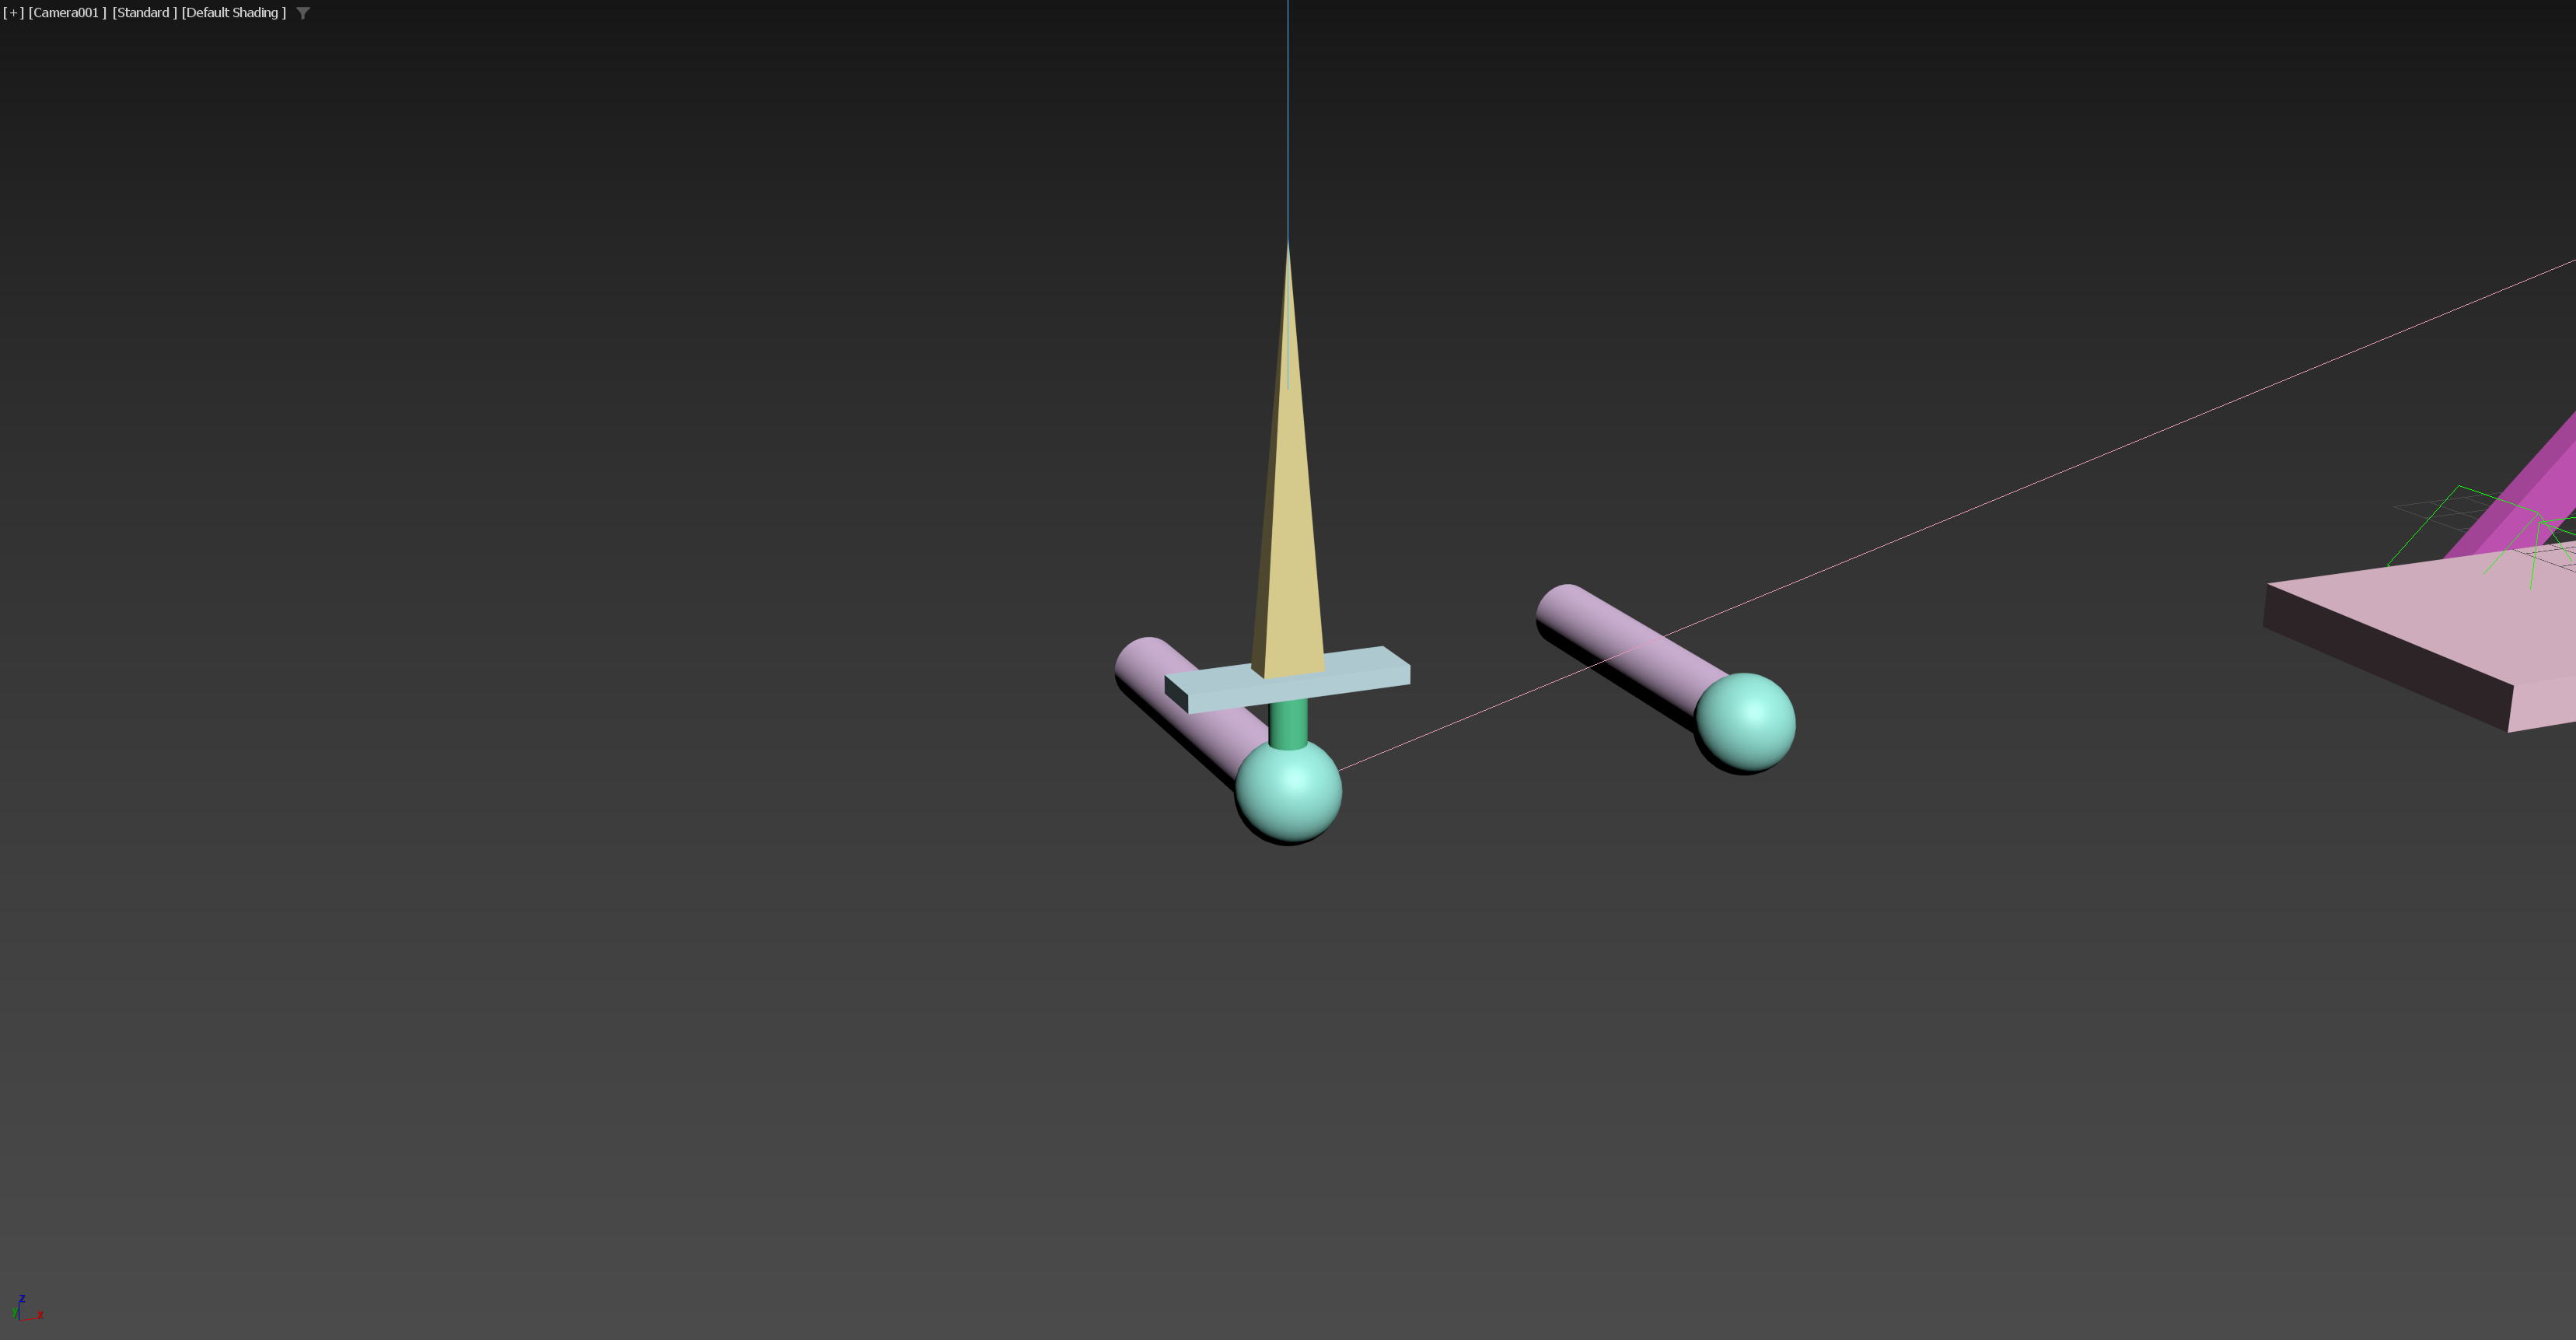
\includegraphics[width=\textwidth]{imagenes/resultado/0.png}
        \caption{Animación en el instante 0.}
    \end{subfigure}
    \hfill
    \begin{subfigure}[t]{0.48\textwidth}
        \centering
        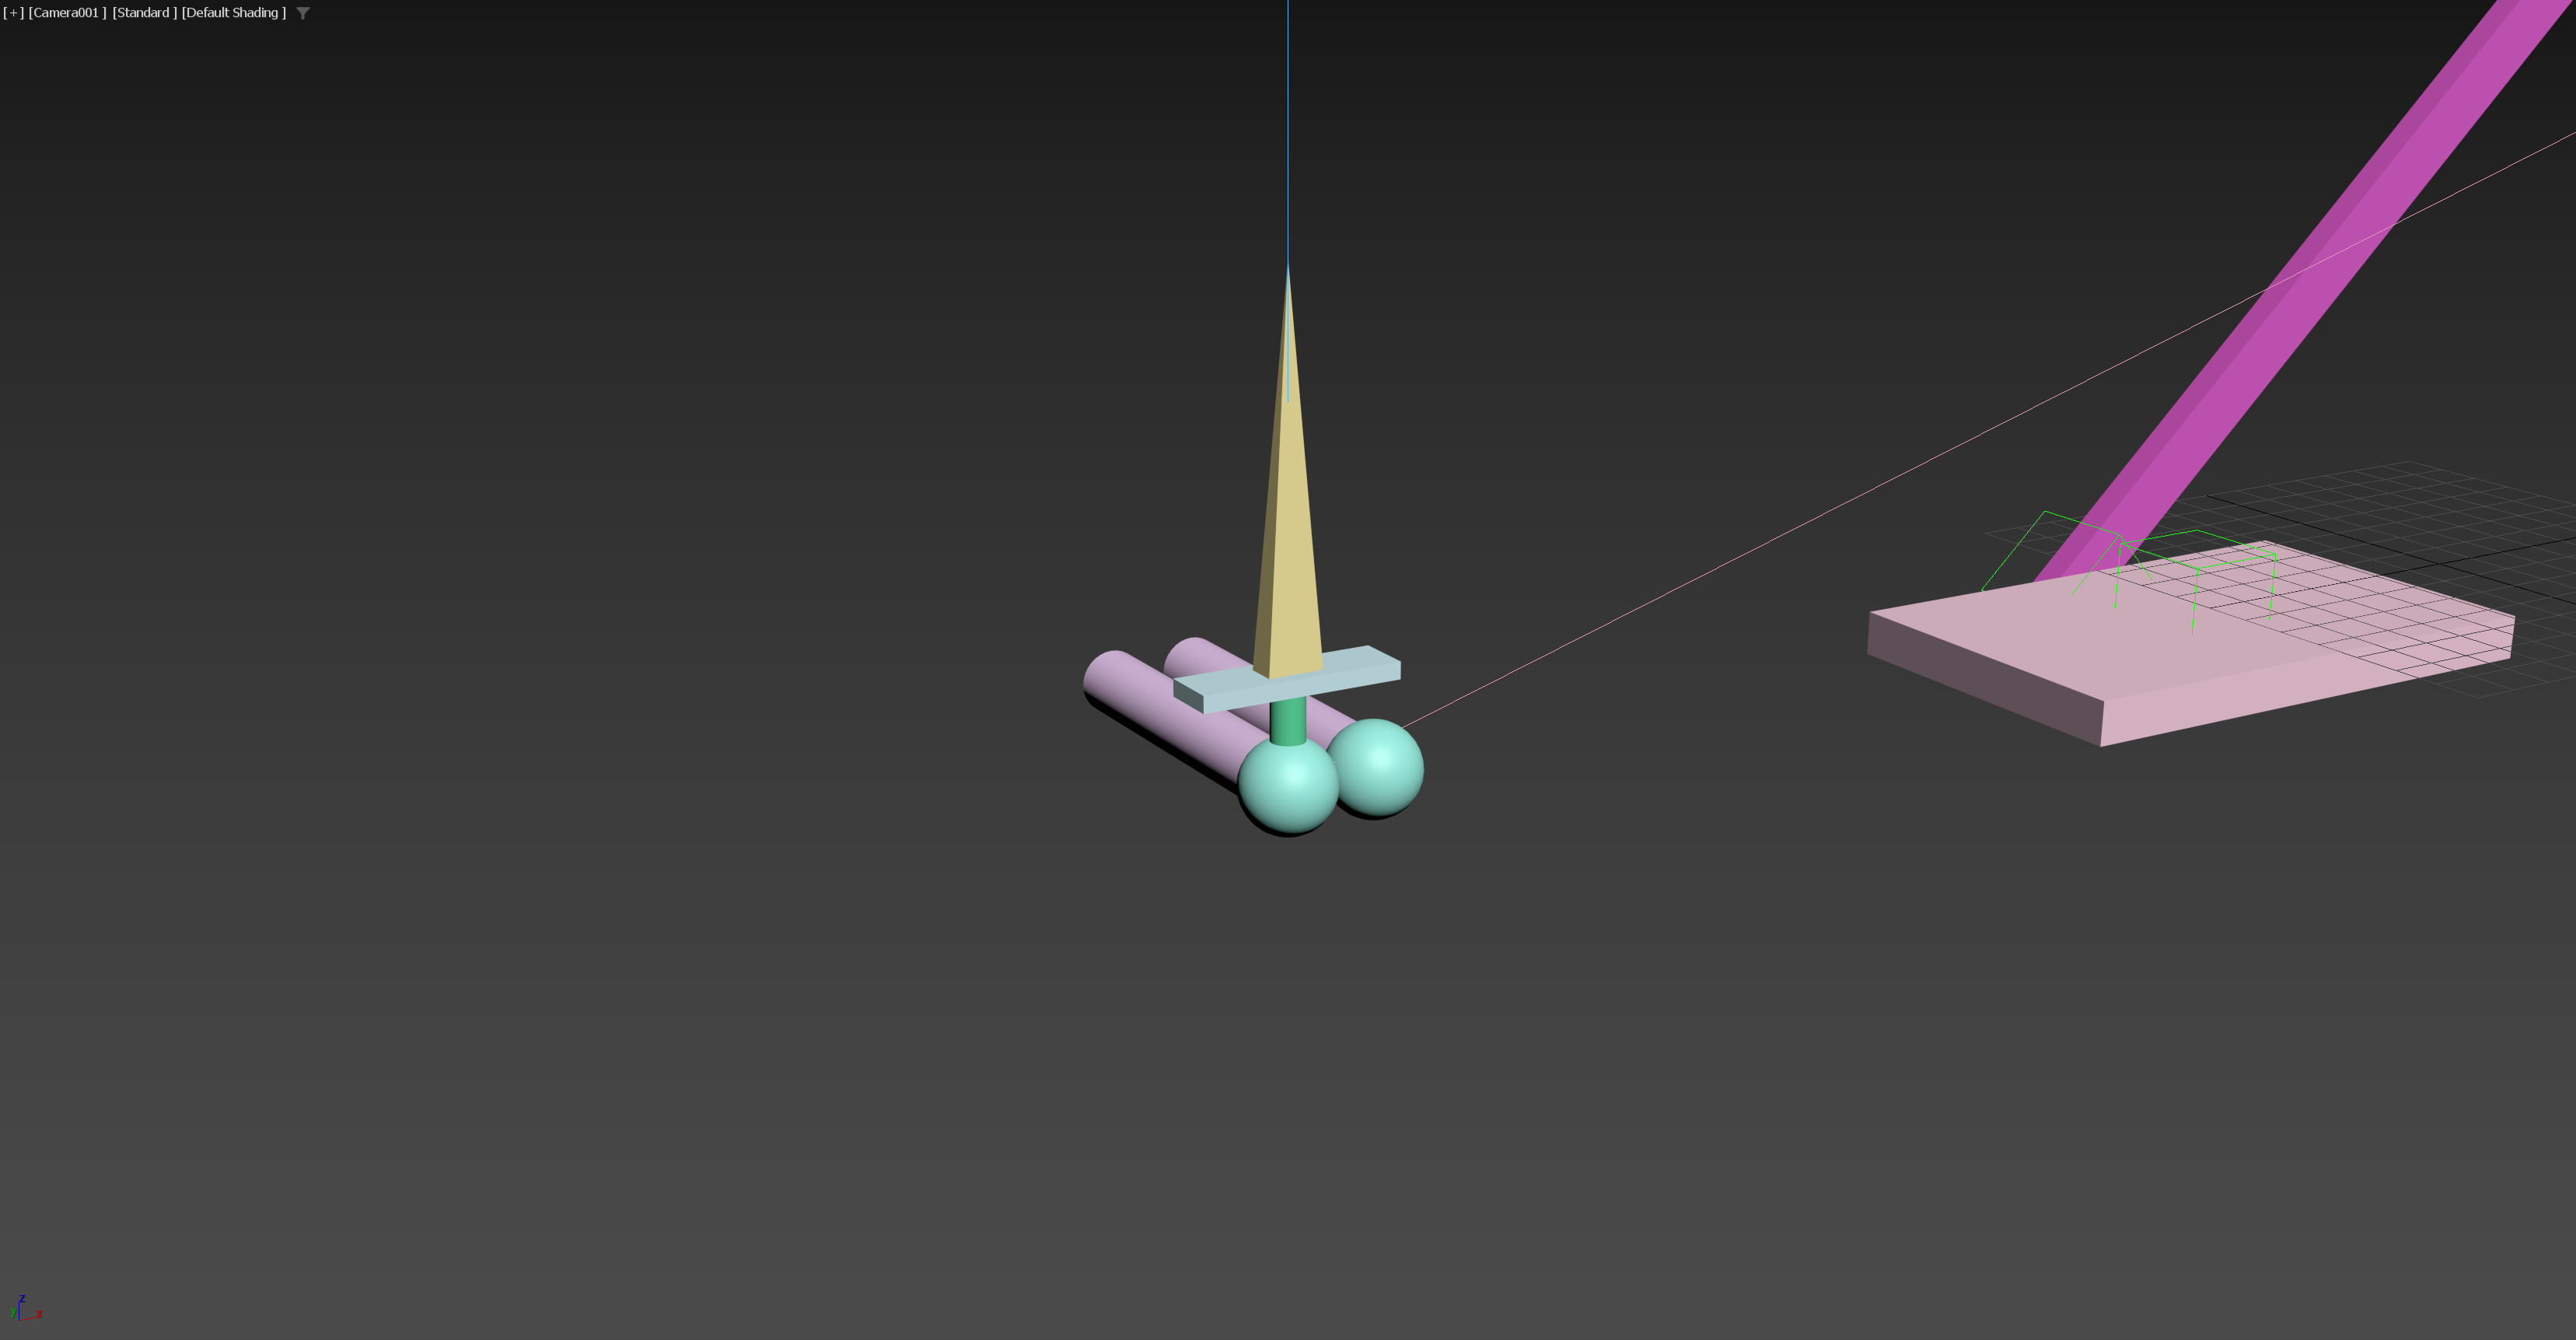
\includegraphics[width=\textwidth]{imagenes/resultado/20.png}
        \caption{Animación en el instante 20.}
    \end{subfigure}
    \hfill
    \begin{subfigure}[t]{0.48\textwidth}
        \centering
        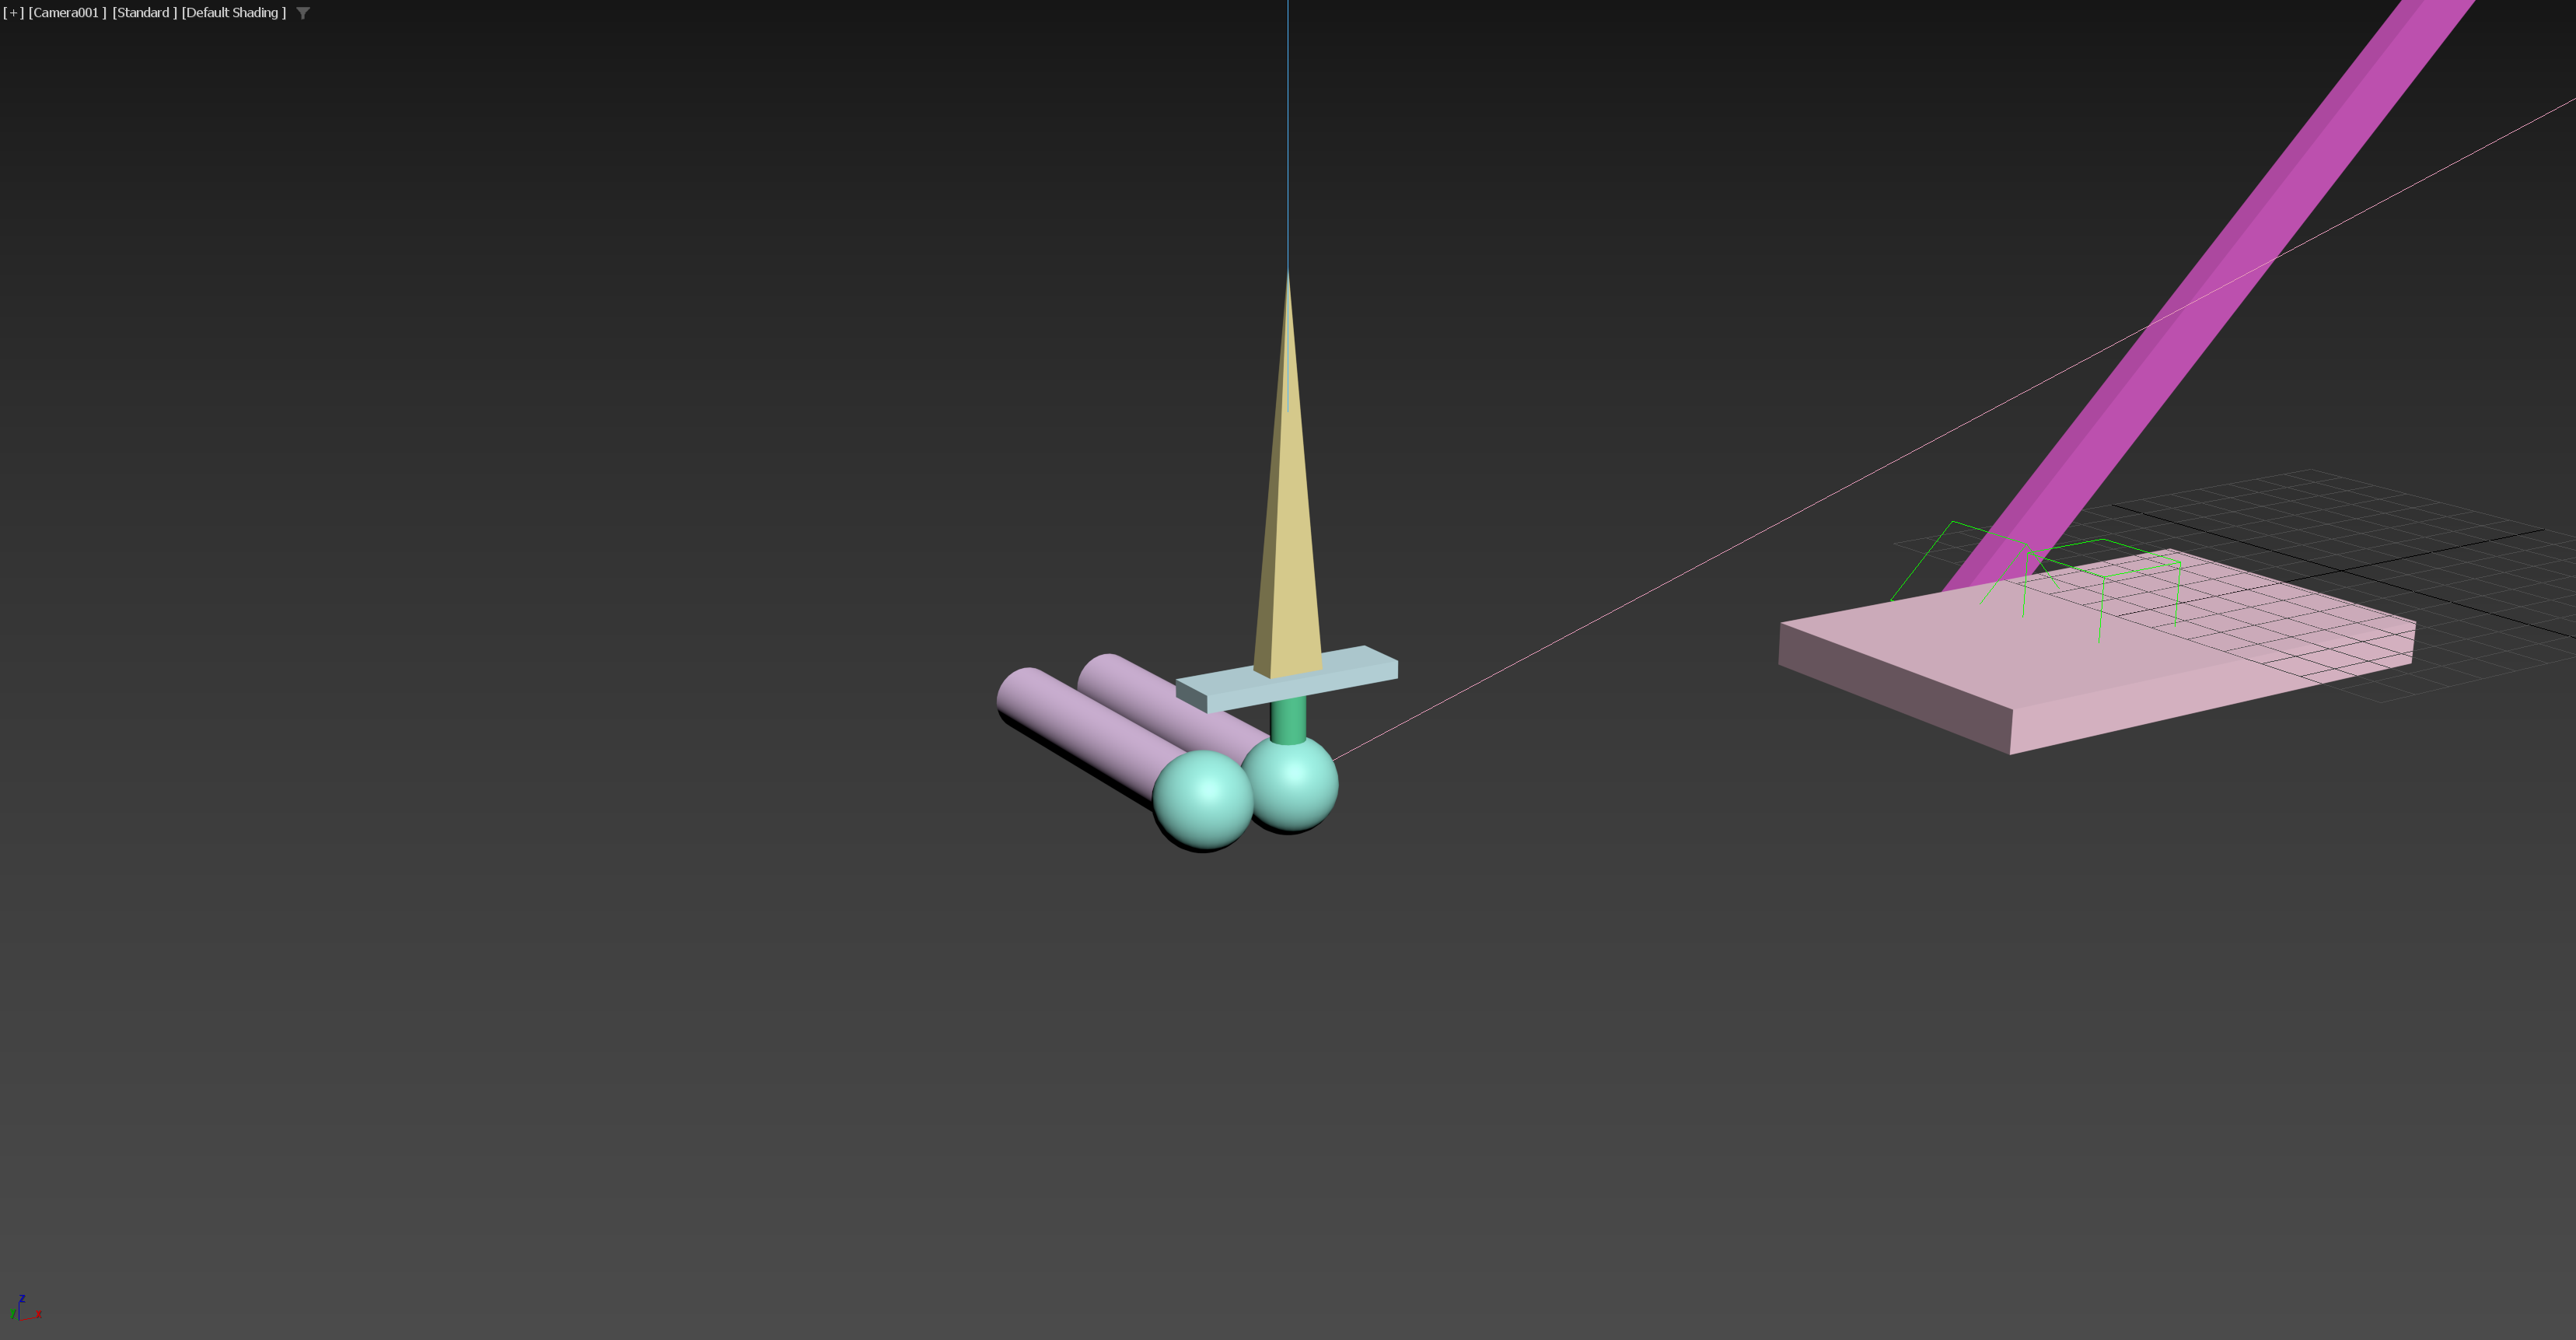
\includegraphics[width=\textwidth]{imagenes/resultado/27y30.png}
        \caption{Animación en los instantes 27 y 30.}
    \end{subfigure}
    \hfill
    \begin{subfigure}[t]{0.48\textwidth}
        \centering
        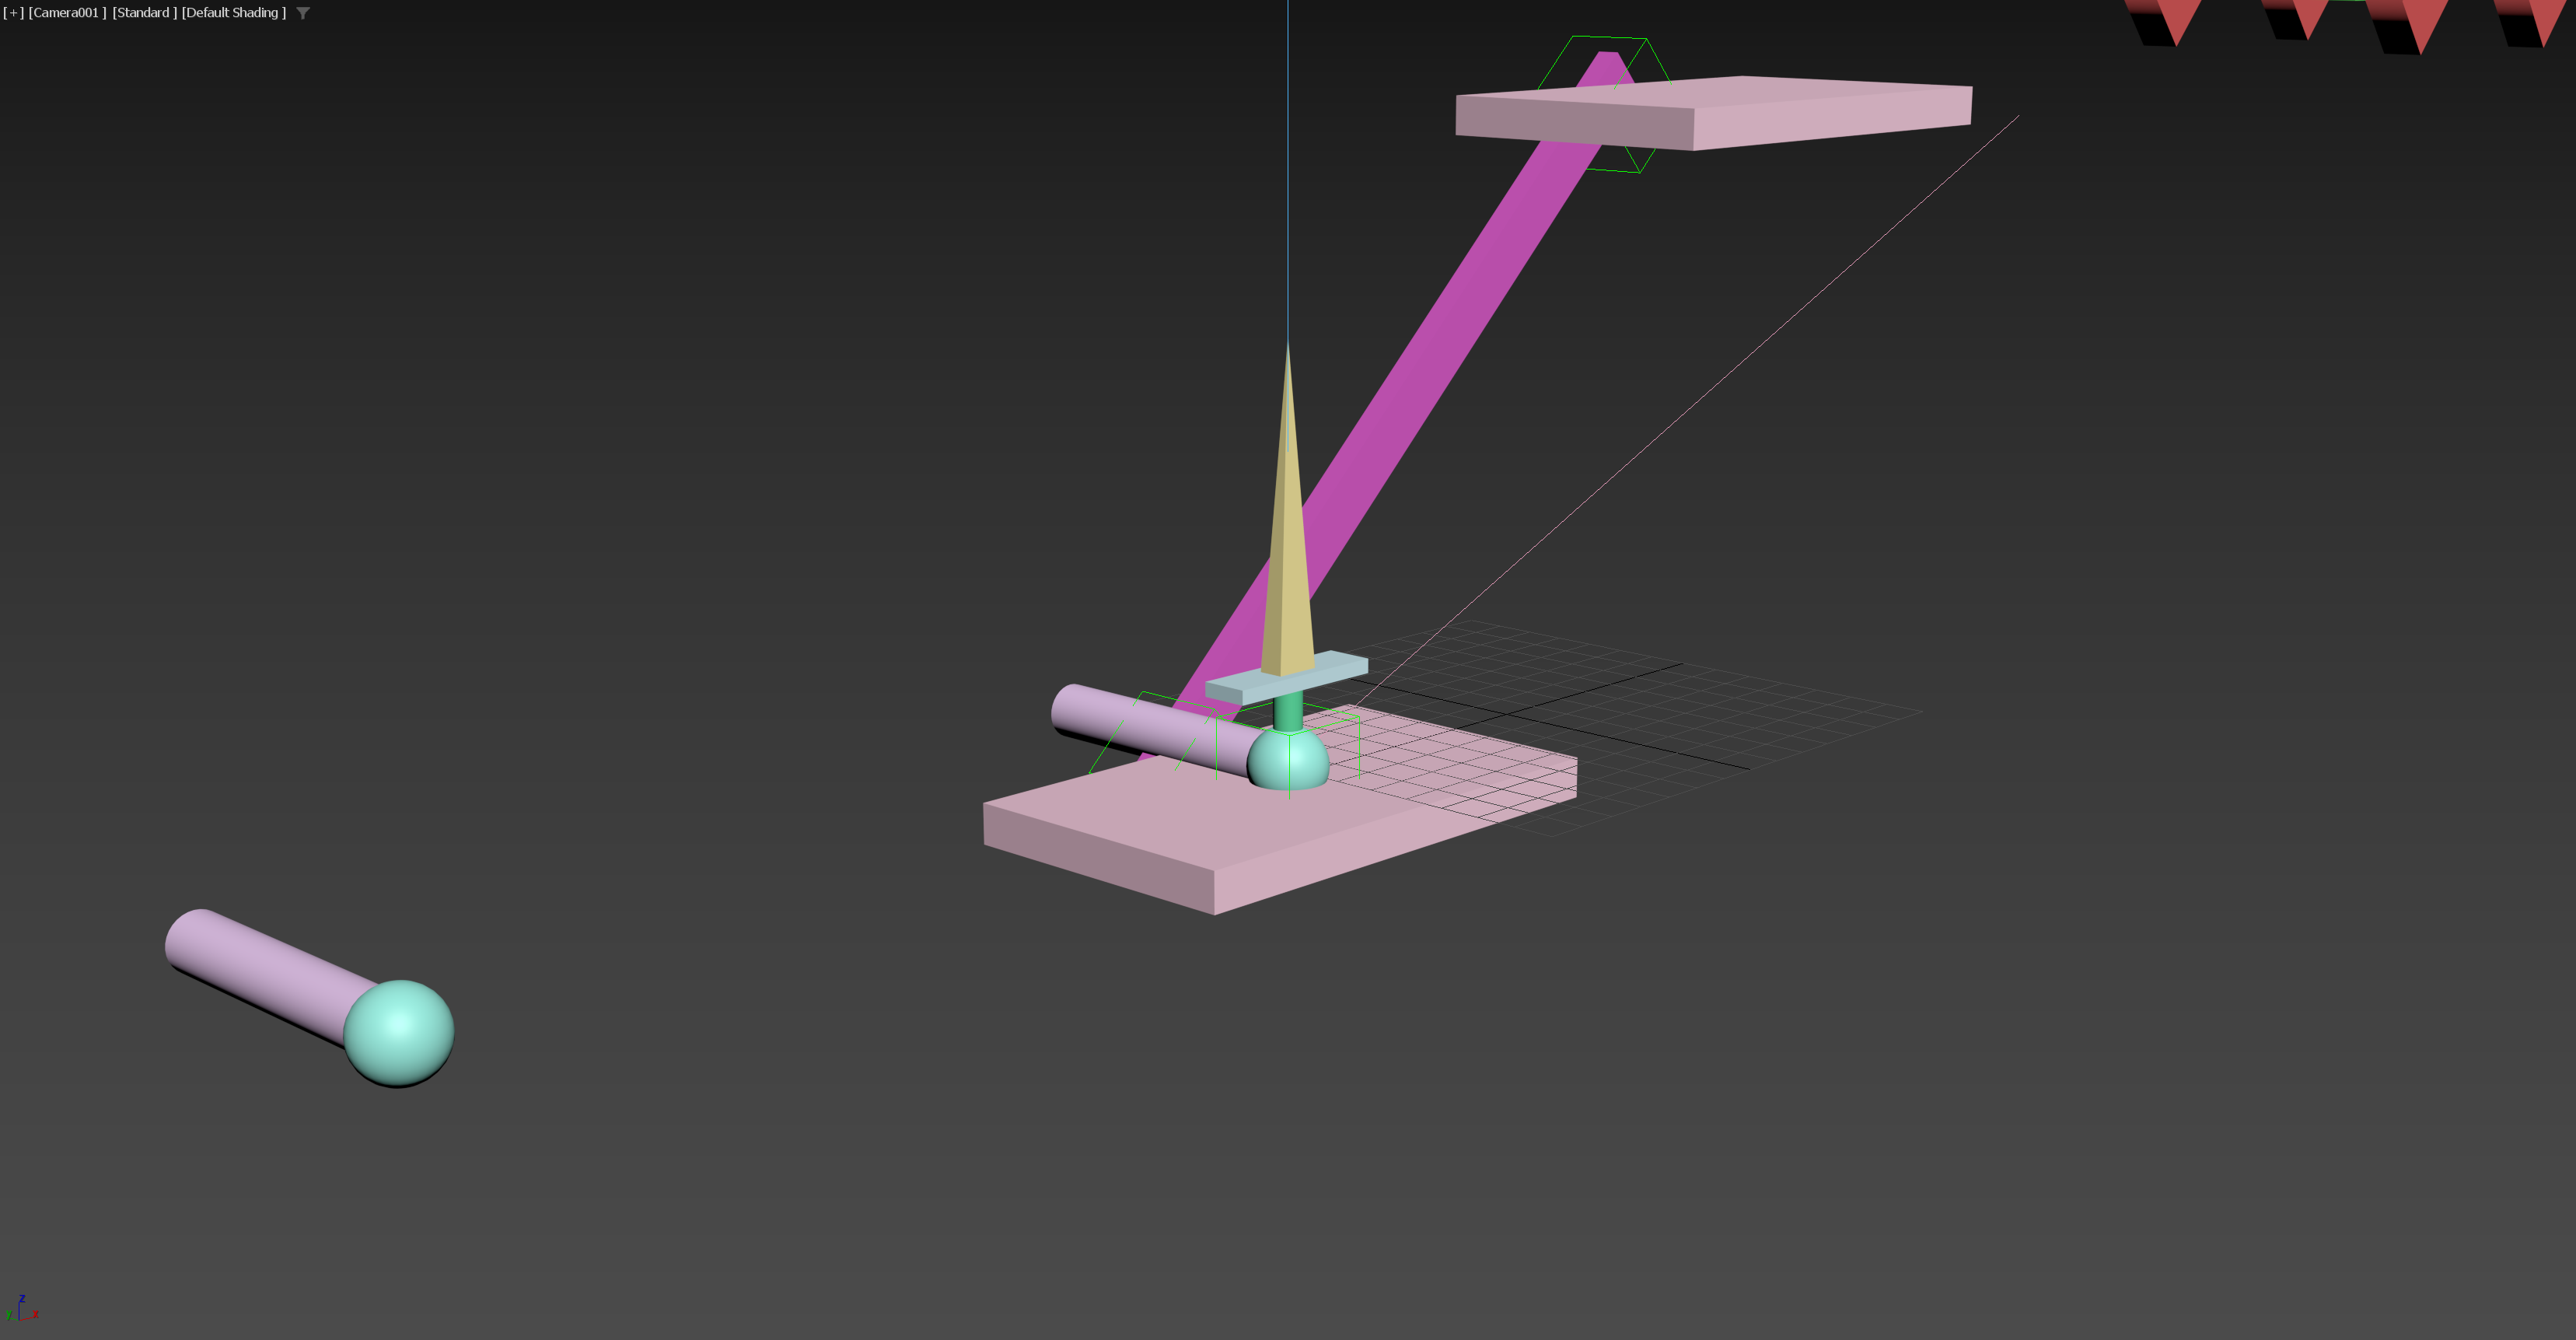
\includegraphics[width=\textwidth]{imagenes/resultado/65.png}
        \caption{Animación en el instante 65.}
    \end{subfigure}
    \hfill
    \begin{subfigure}[t]{0.48\textwidth}
        \centering
        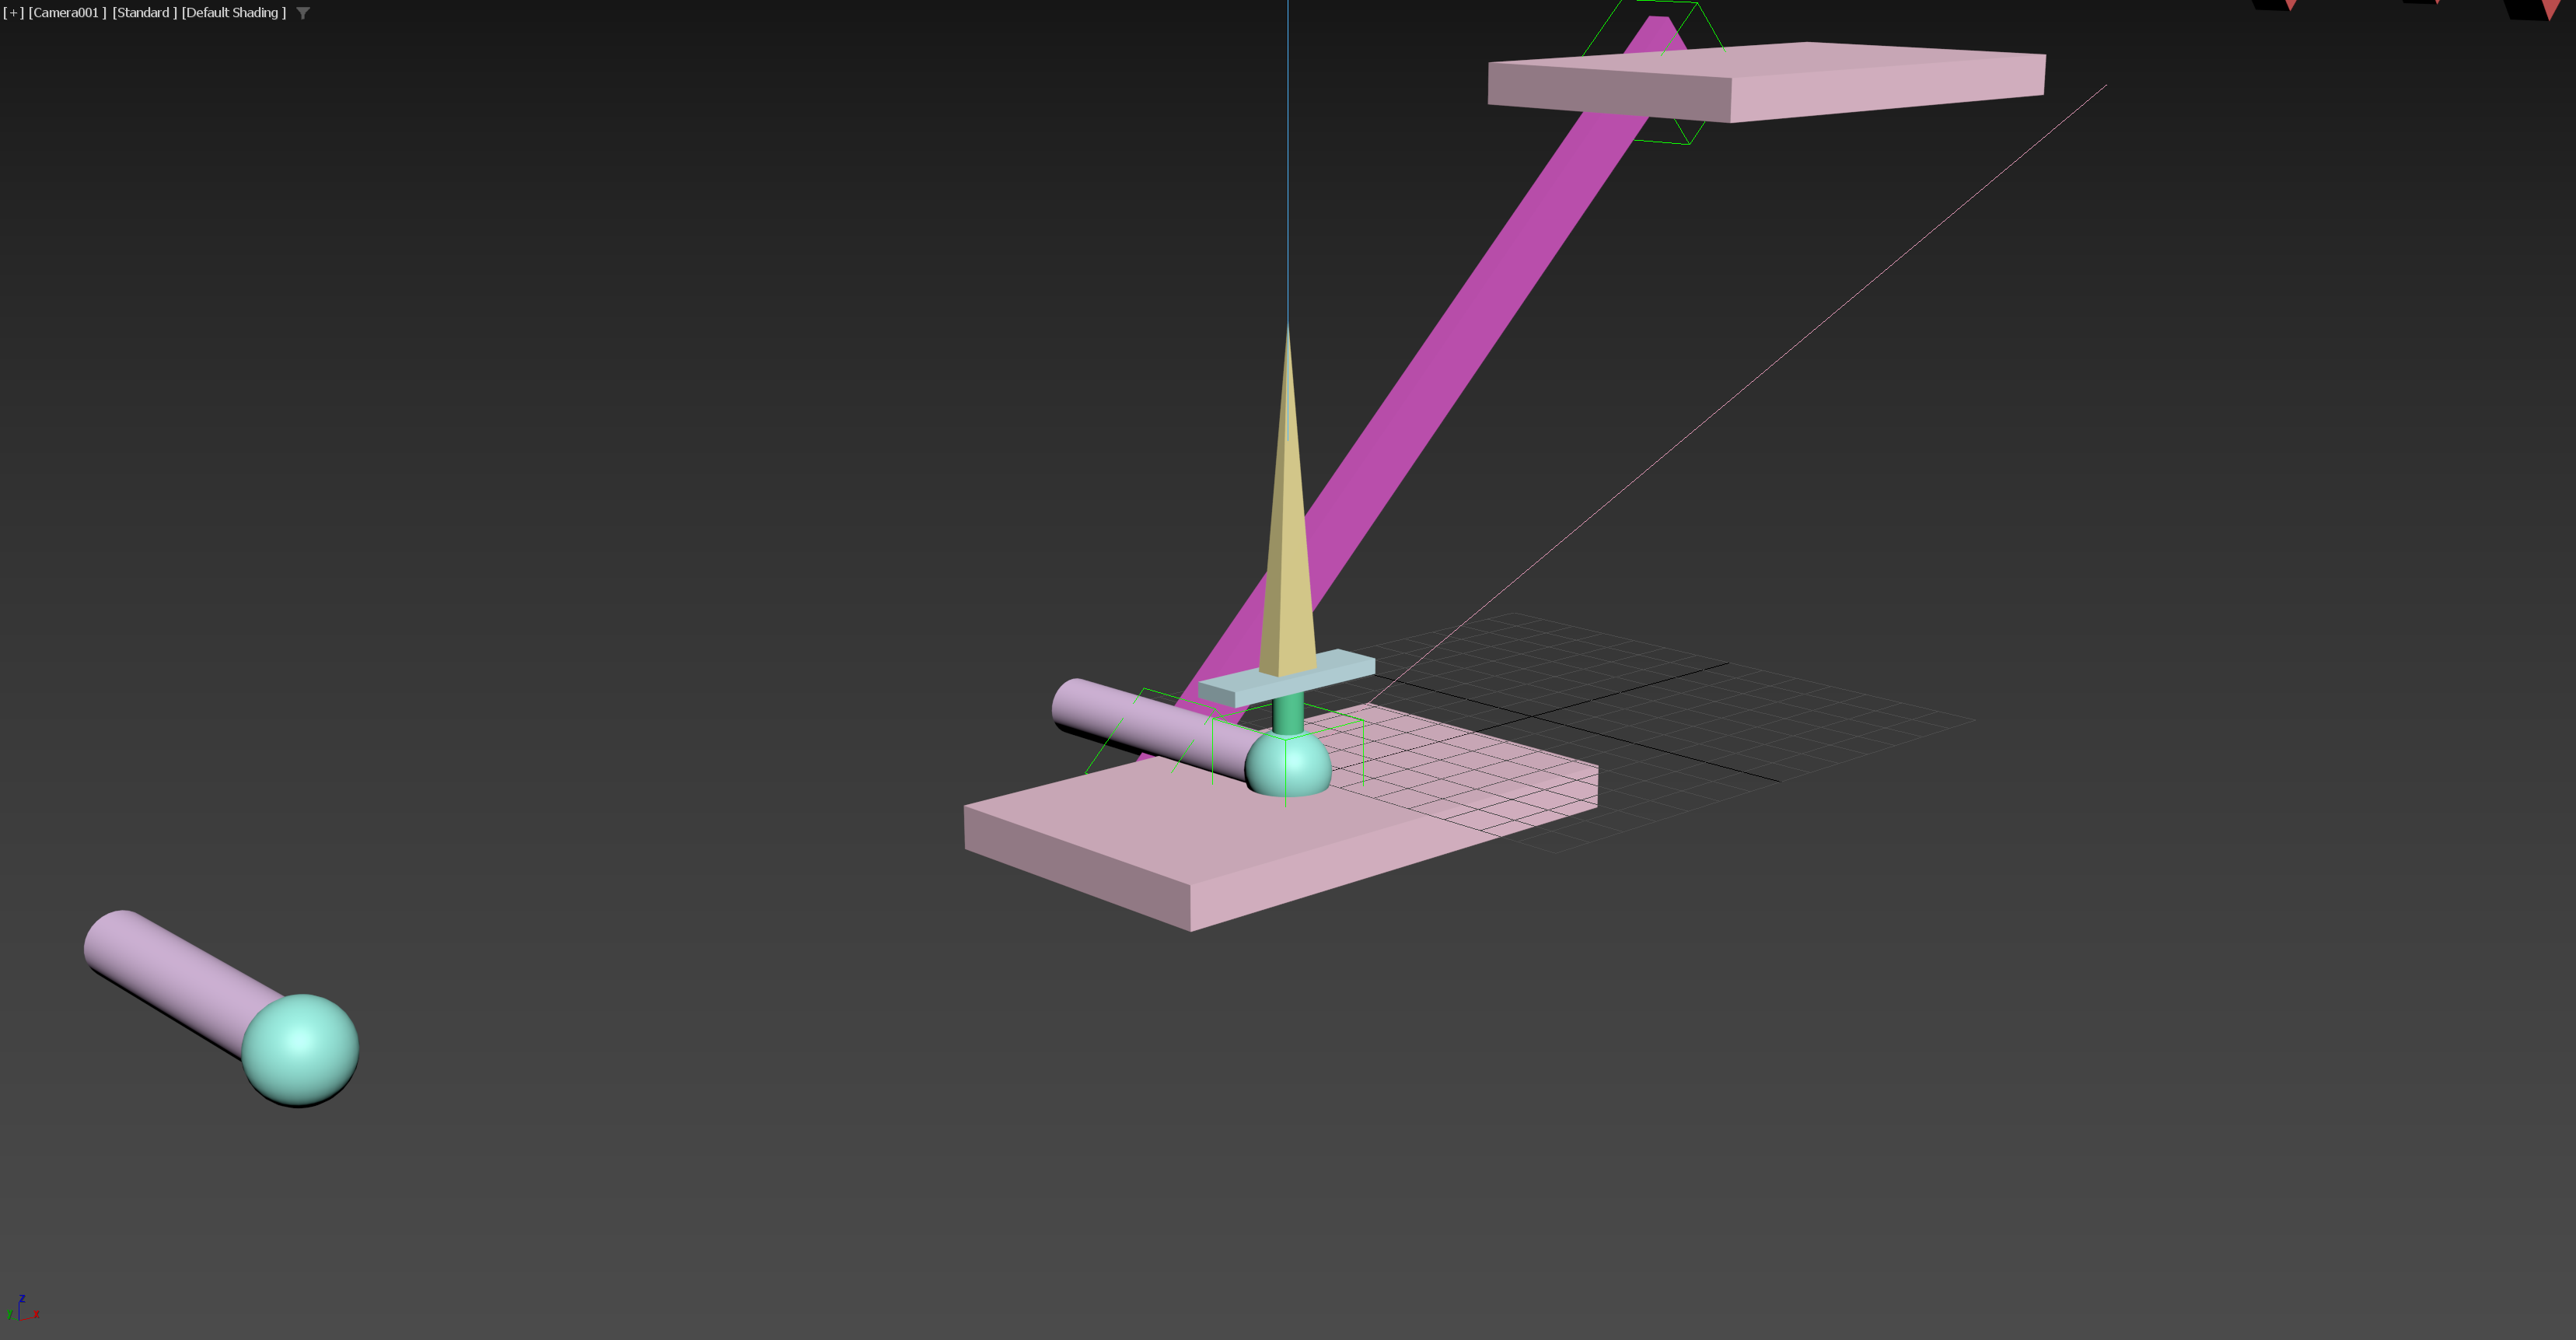
\includegraphics[width=\textwidth]{imagenes/resultado/70.png}
        \caption{Animación en el instante 70.}
    \end{subfigure}
    \hfill
    \begin{subfigure}[t]{0.48\textwidth}
        \centering
        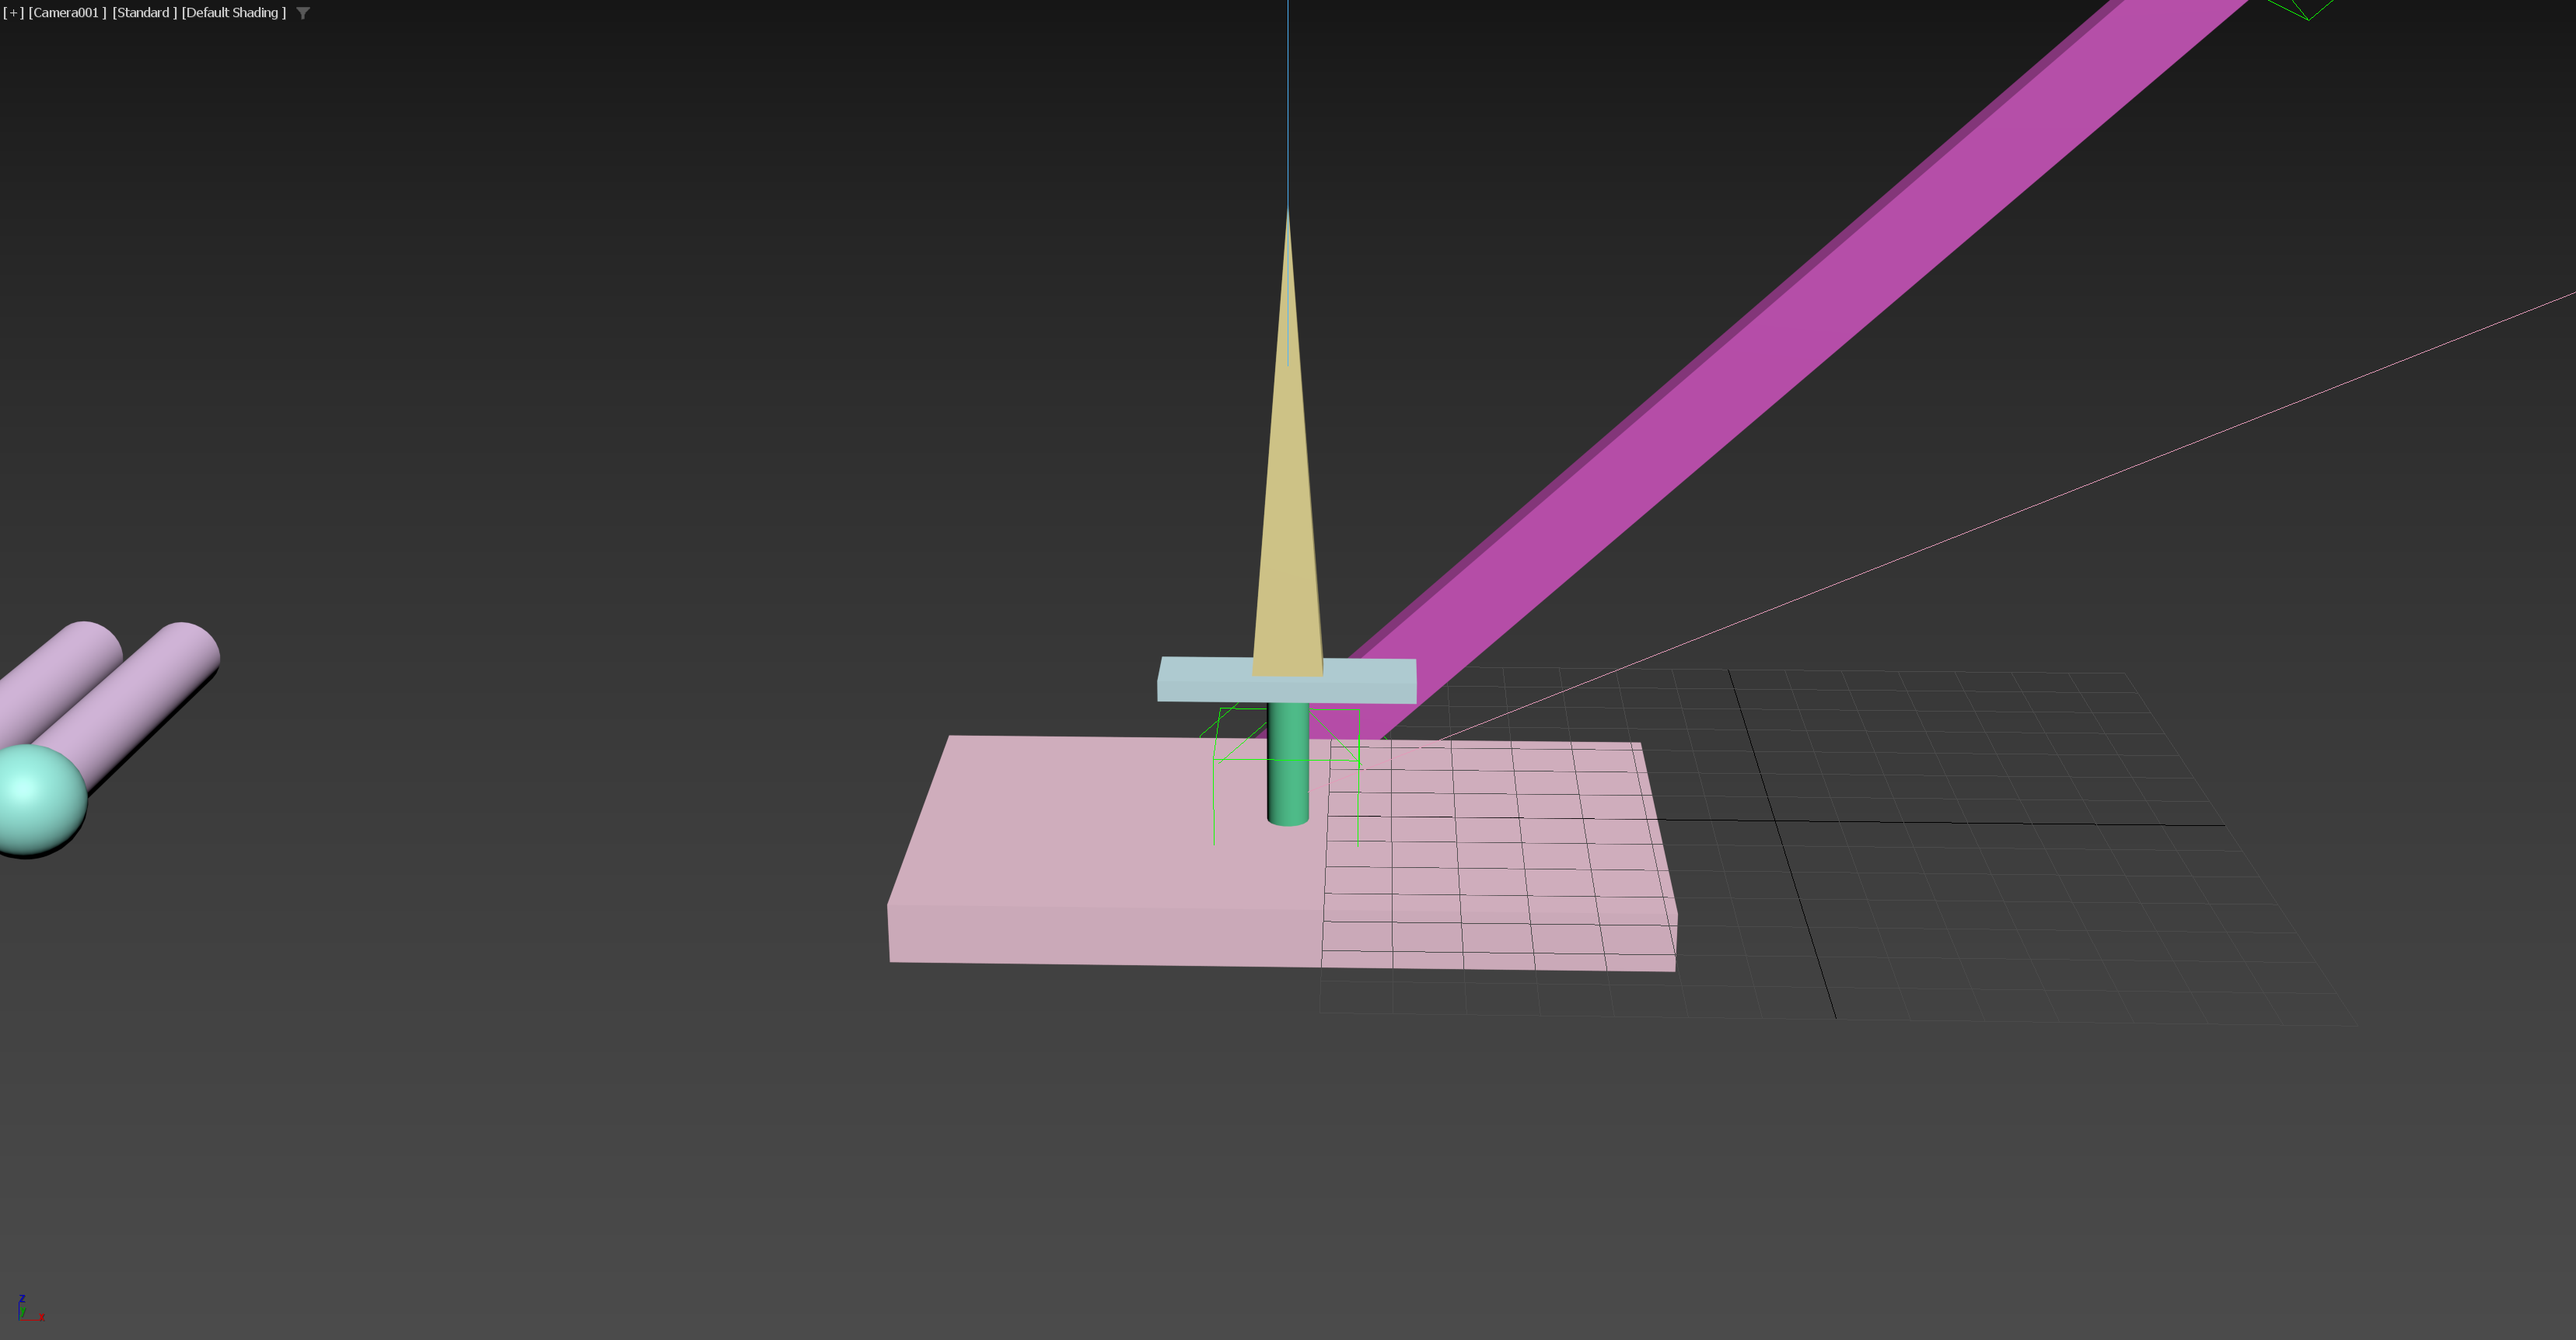
\includegraphics[width=\textwidth]{imagenes/resultado/90.png}
        \caption{Animación en el instante 90.}
    \end{subfigure}
    \hfill
    \begin{subfigure}[t]{0.48\textwidth}
        \centering
        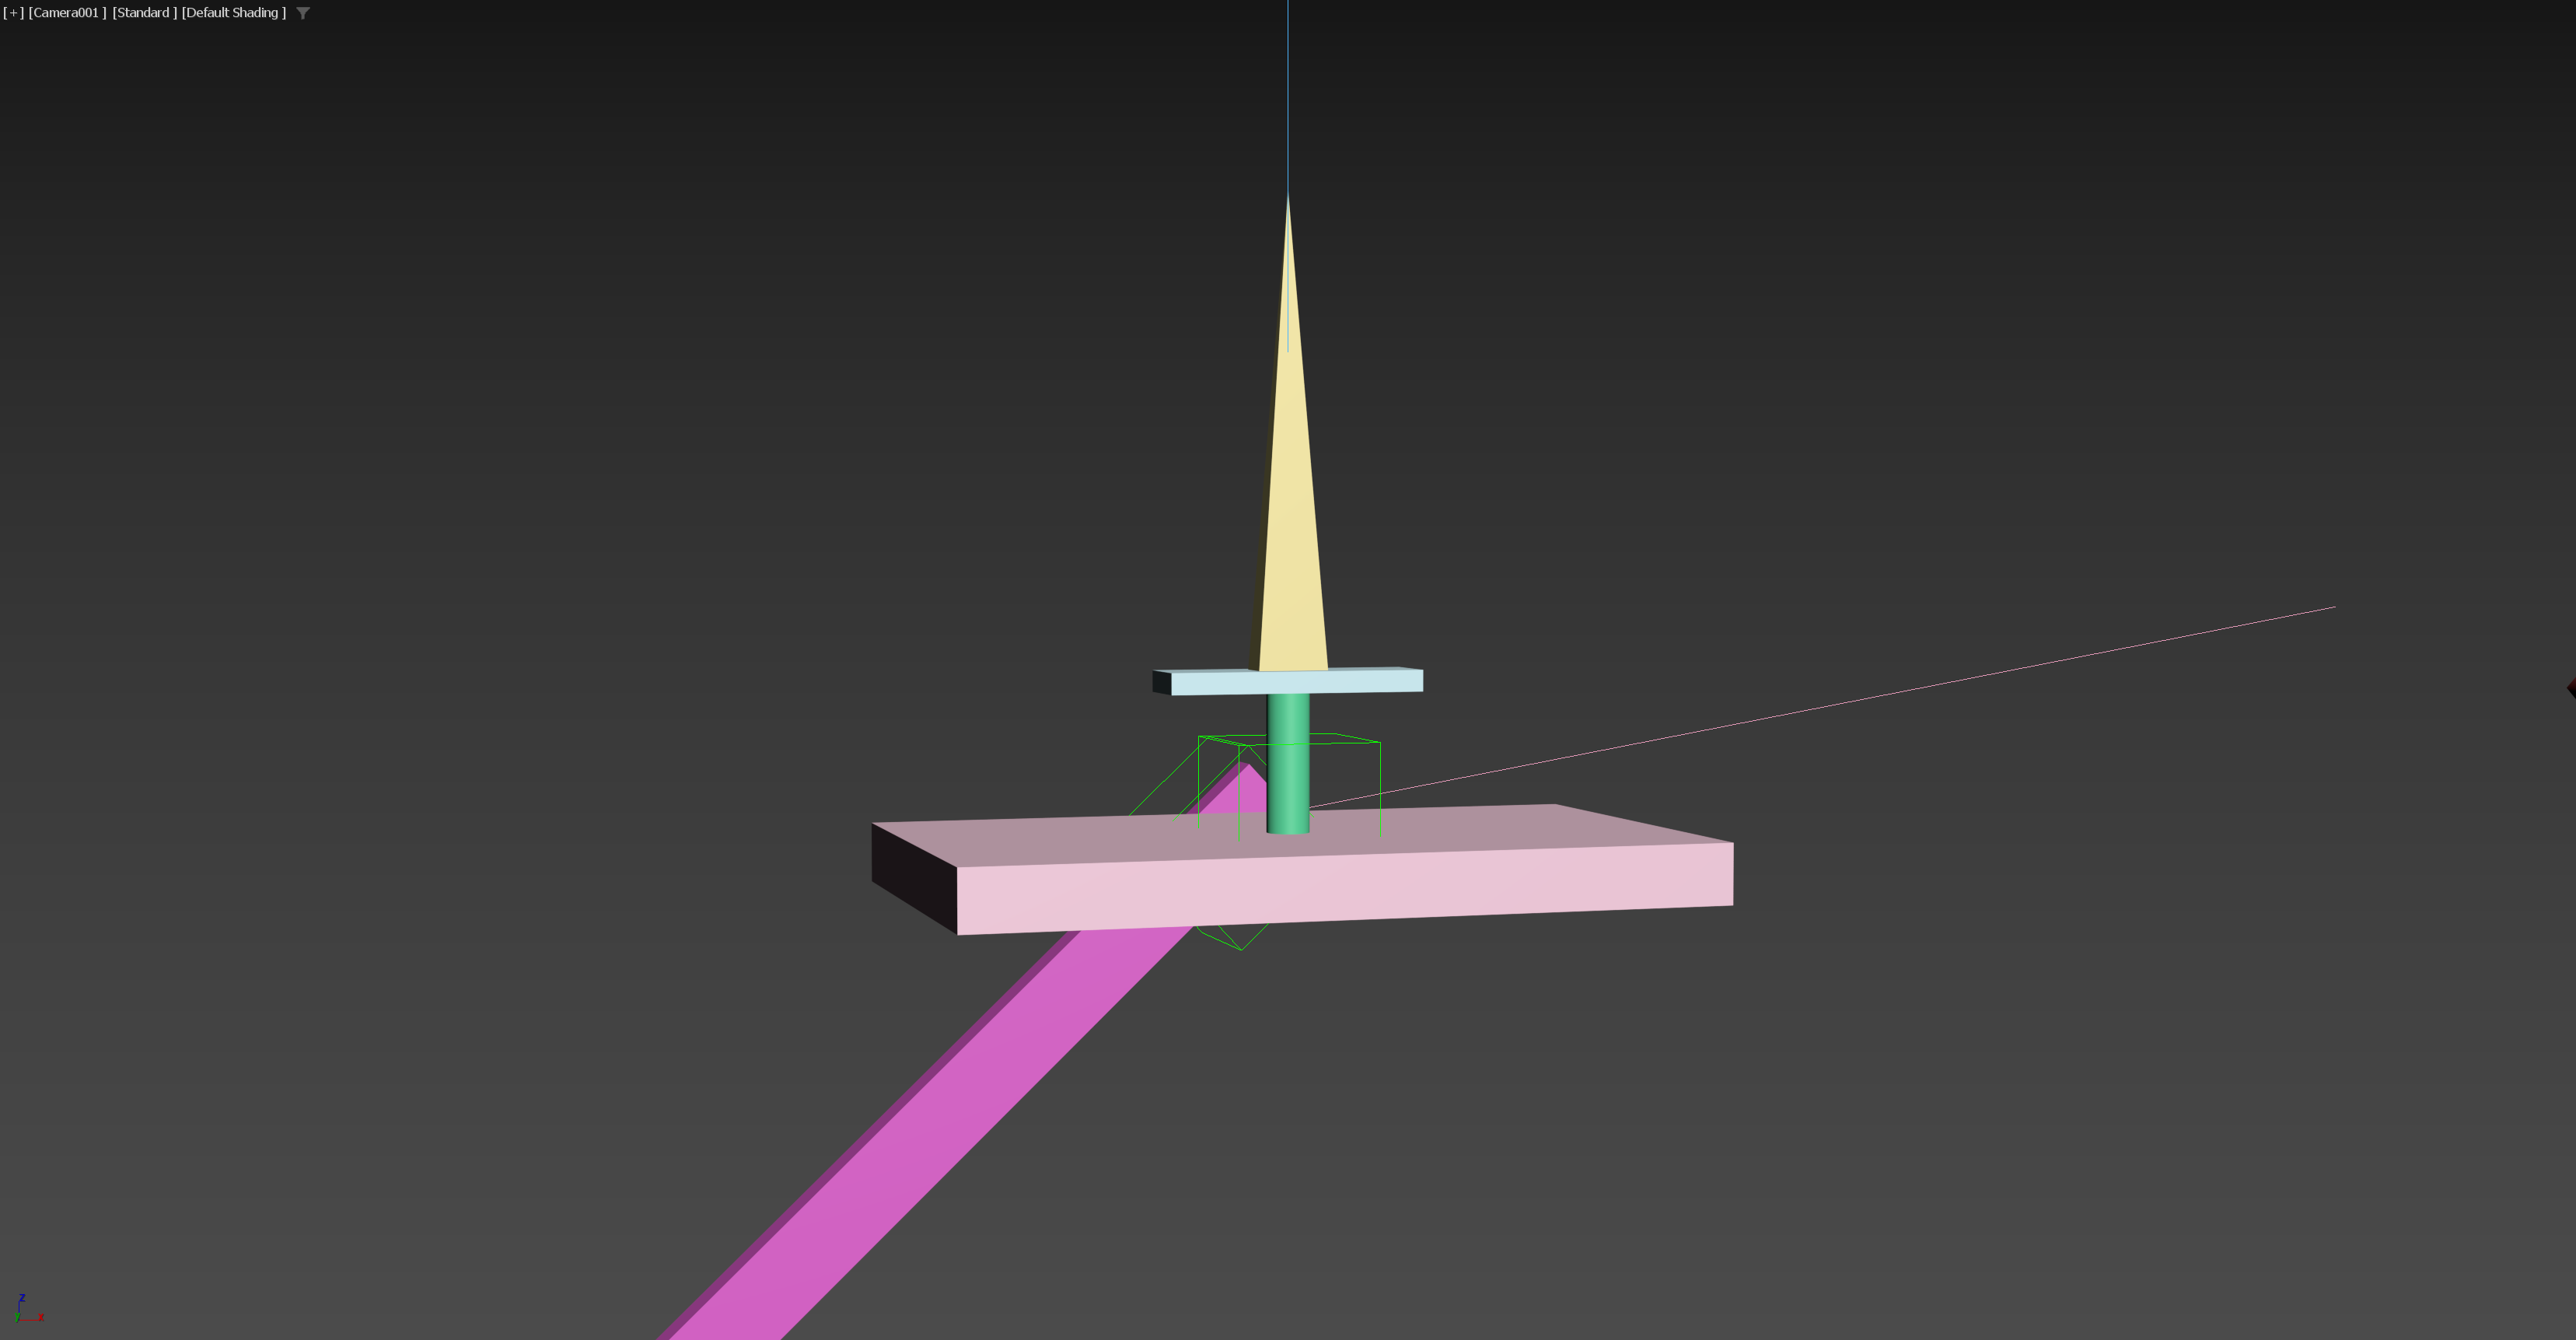
\includegraphics[width=\textwidth]{imagenes/resultado/125.png}
        \caption{Animación en el instante 125.}
    \end{subfigure}
    \hfill
    \begin{subfigure}[t]{0.48\textwidth}
        \centering
        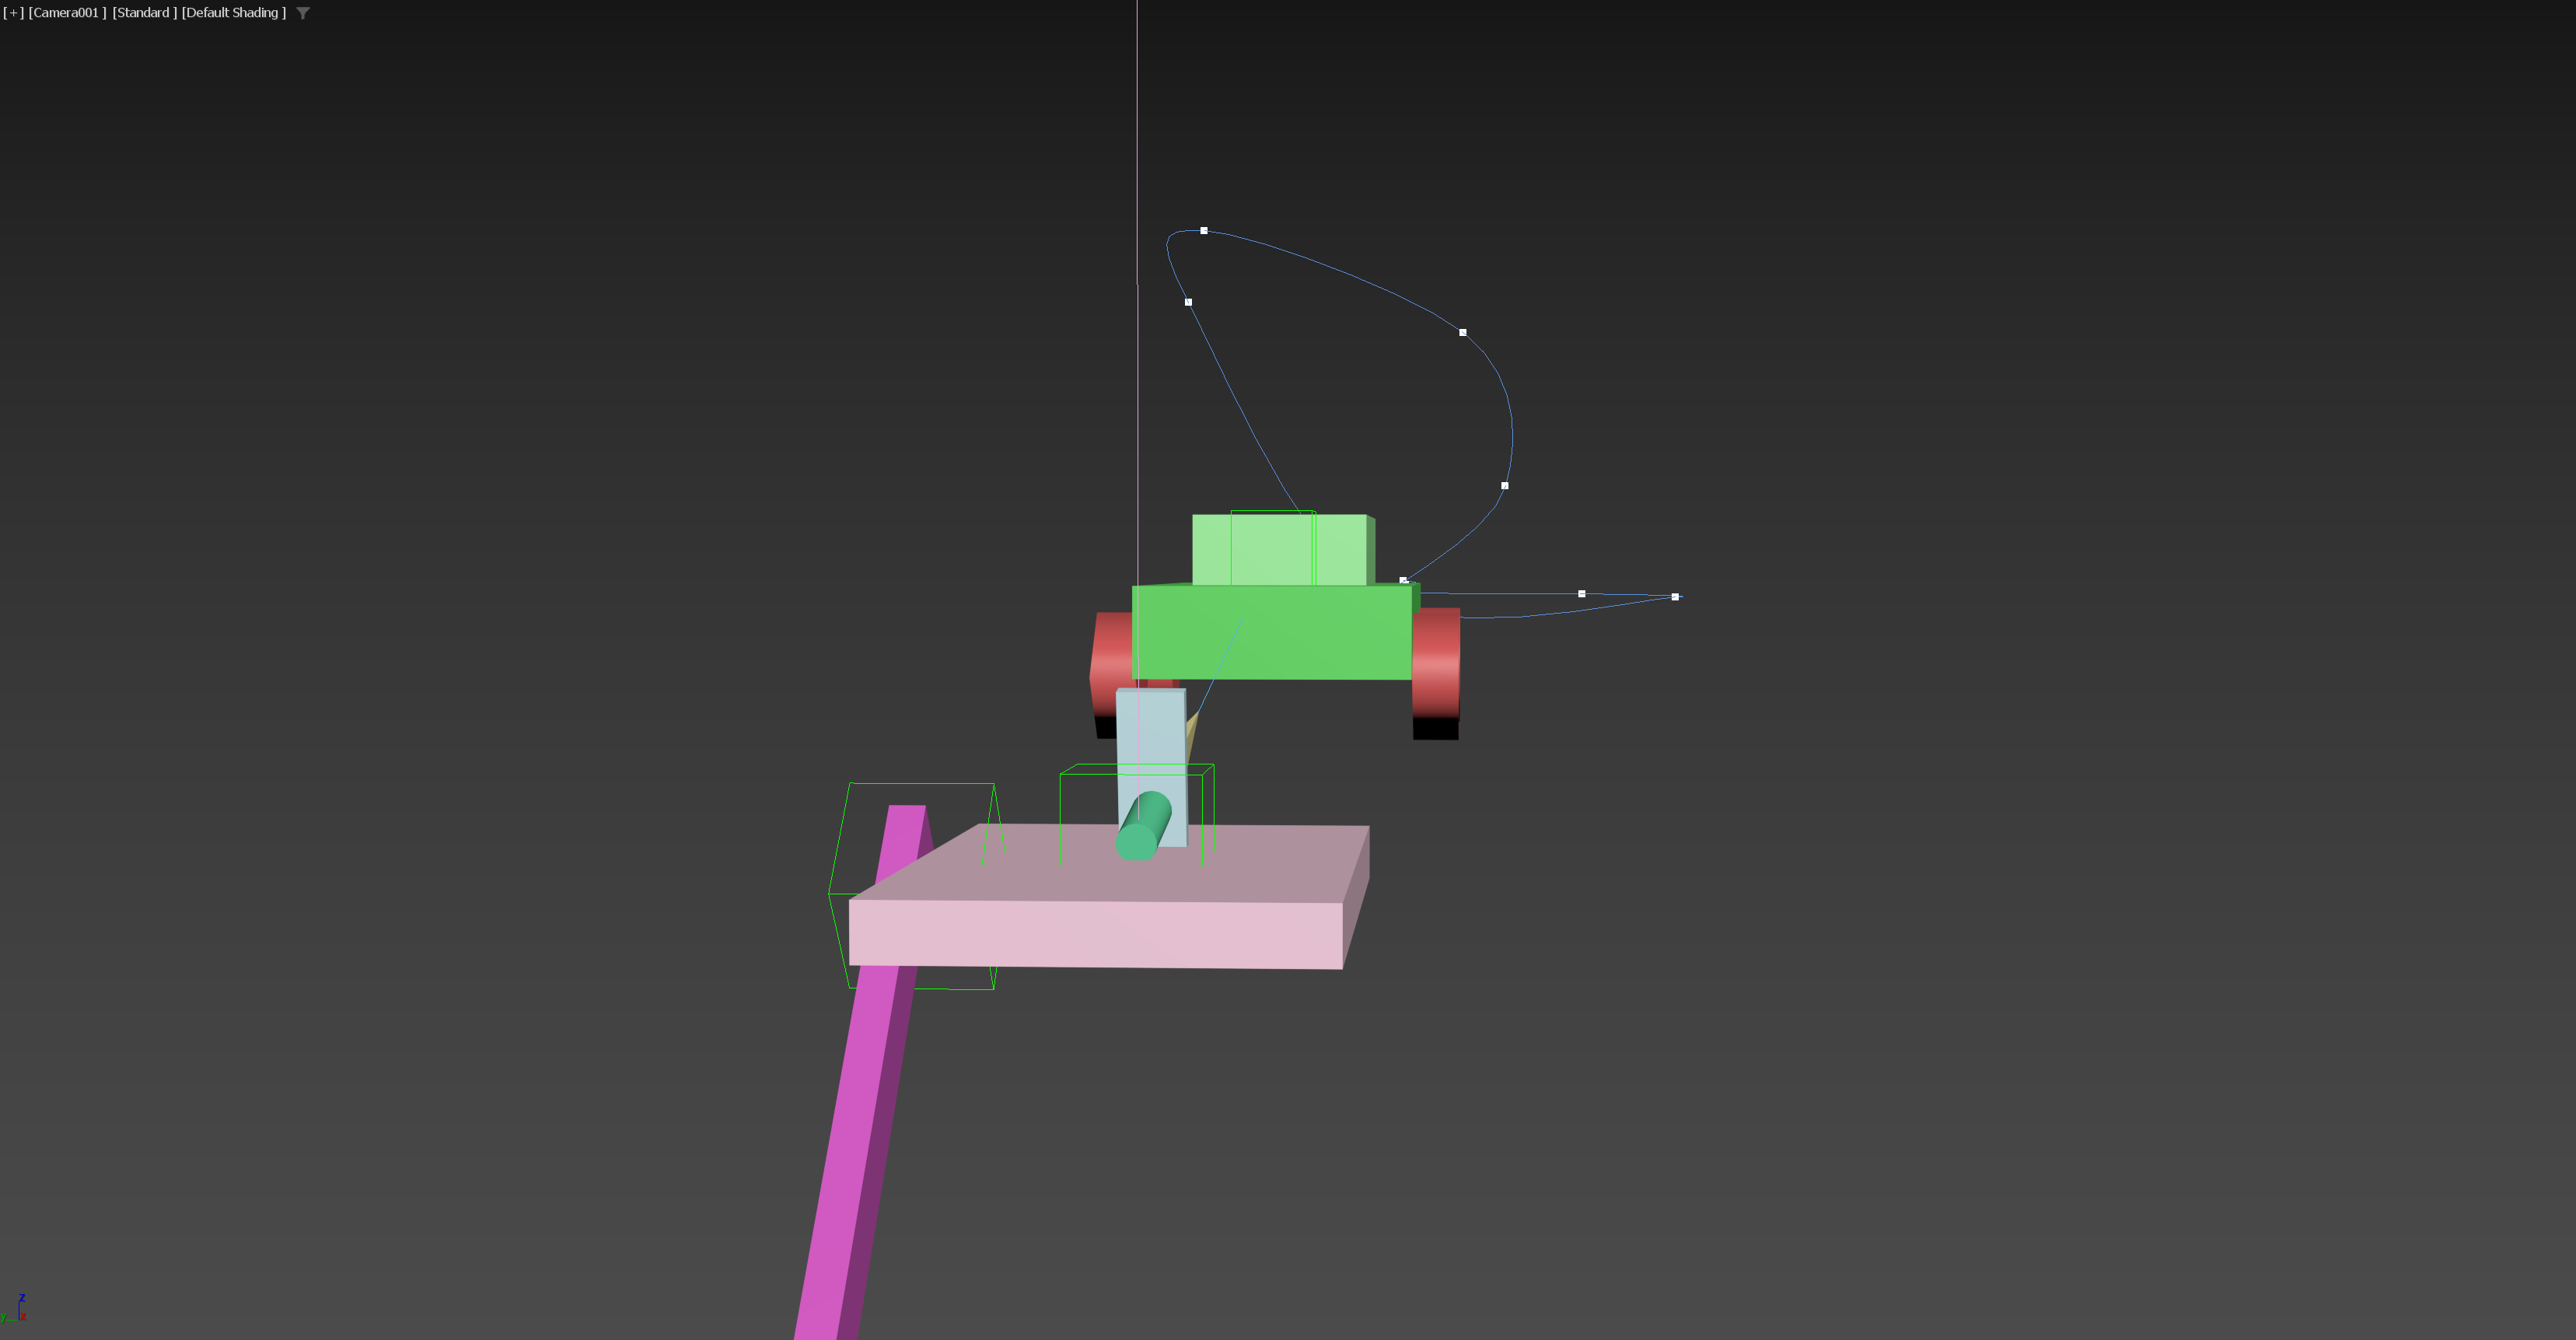
\includegraphics[width=\textwidth]{imagenes/resultado/150.png}
        \caption{Animación en el instante 150.}
    \end{subfigure}
    % \hfill
\end{figure}

\newpage

\begin{figure}[H]\ContinuedFloat
    \centering
    \begin{subfigure}[t]{0.48\textwidth}
        \centering
        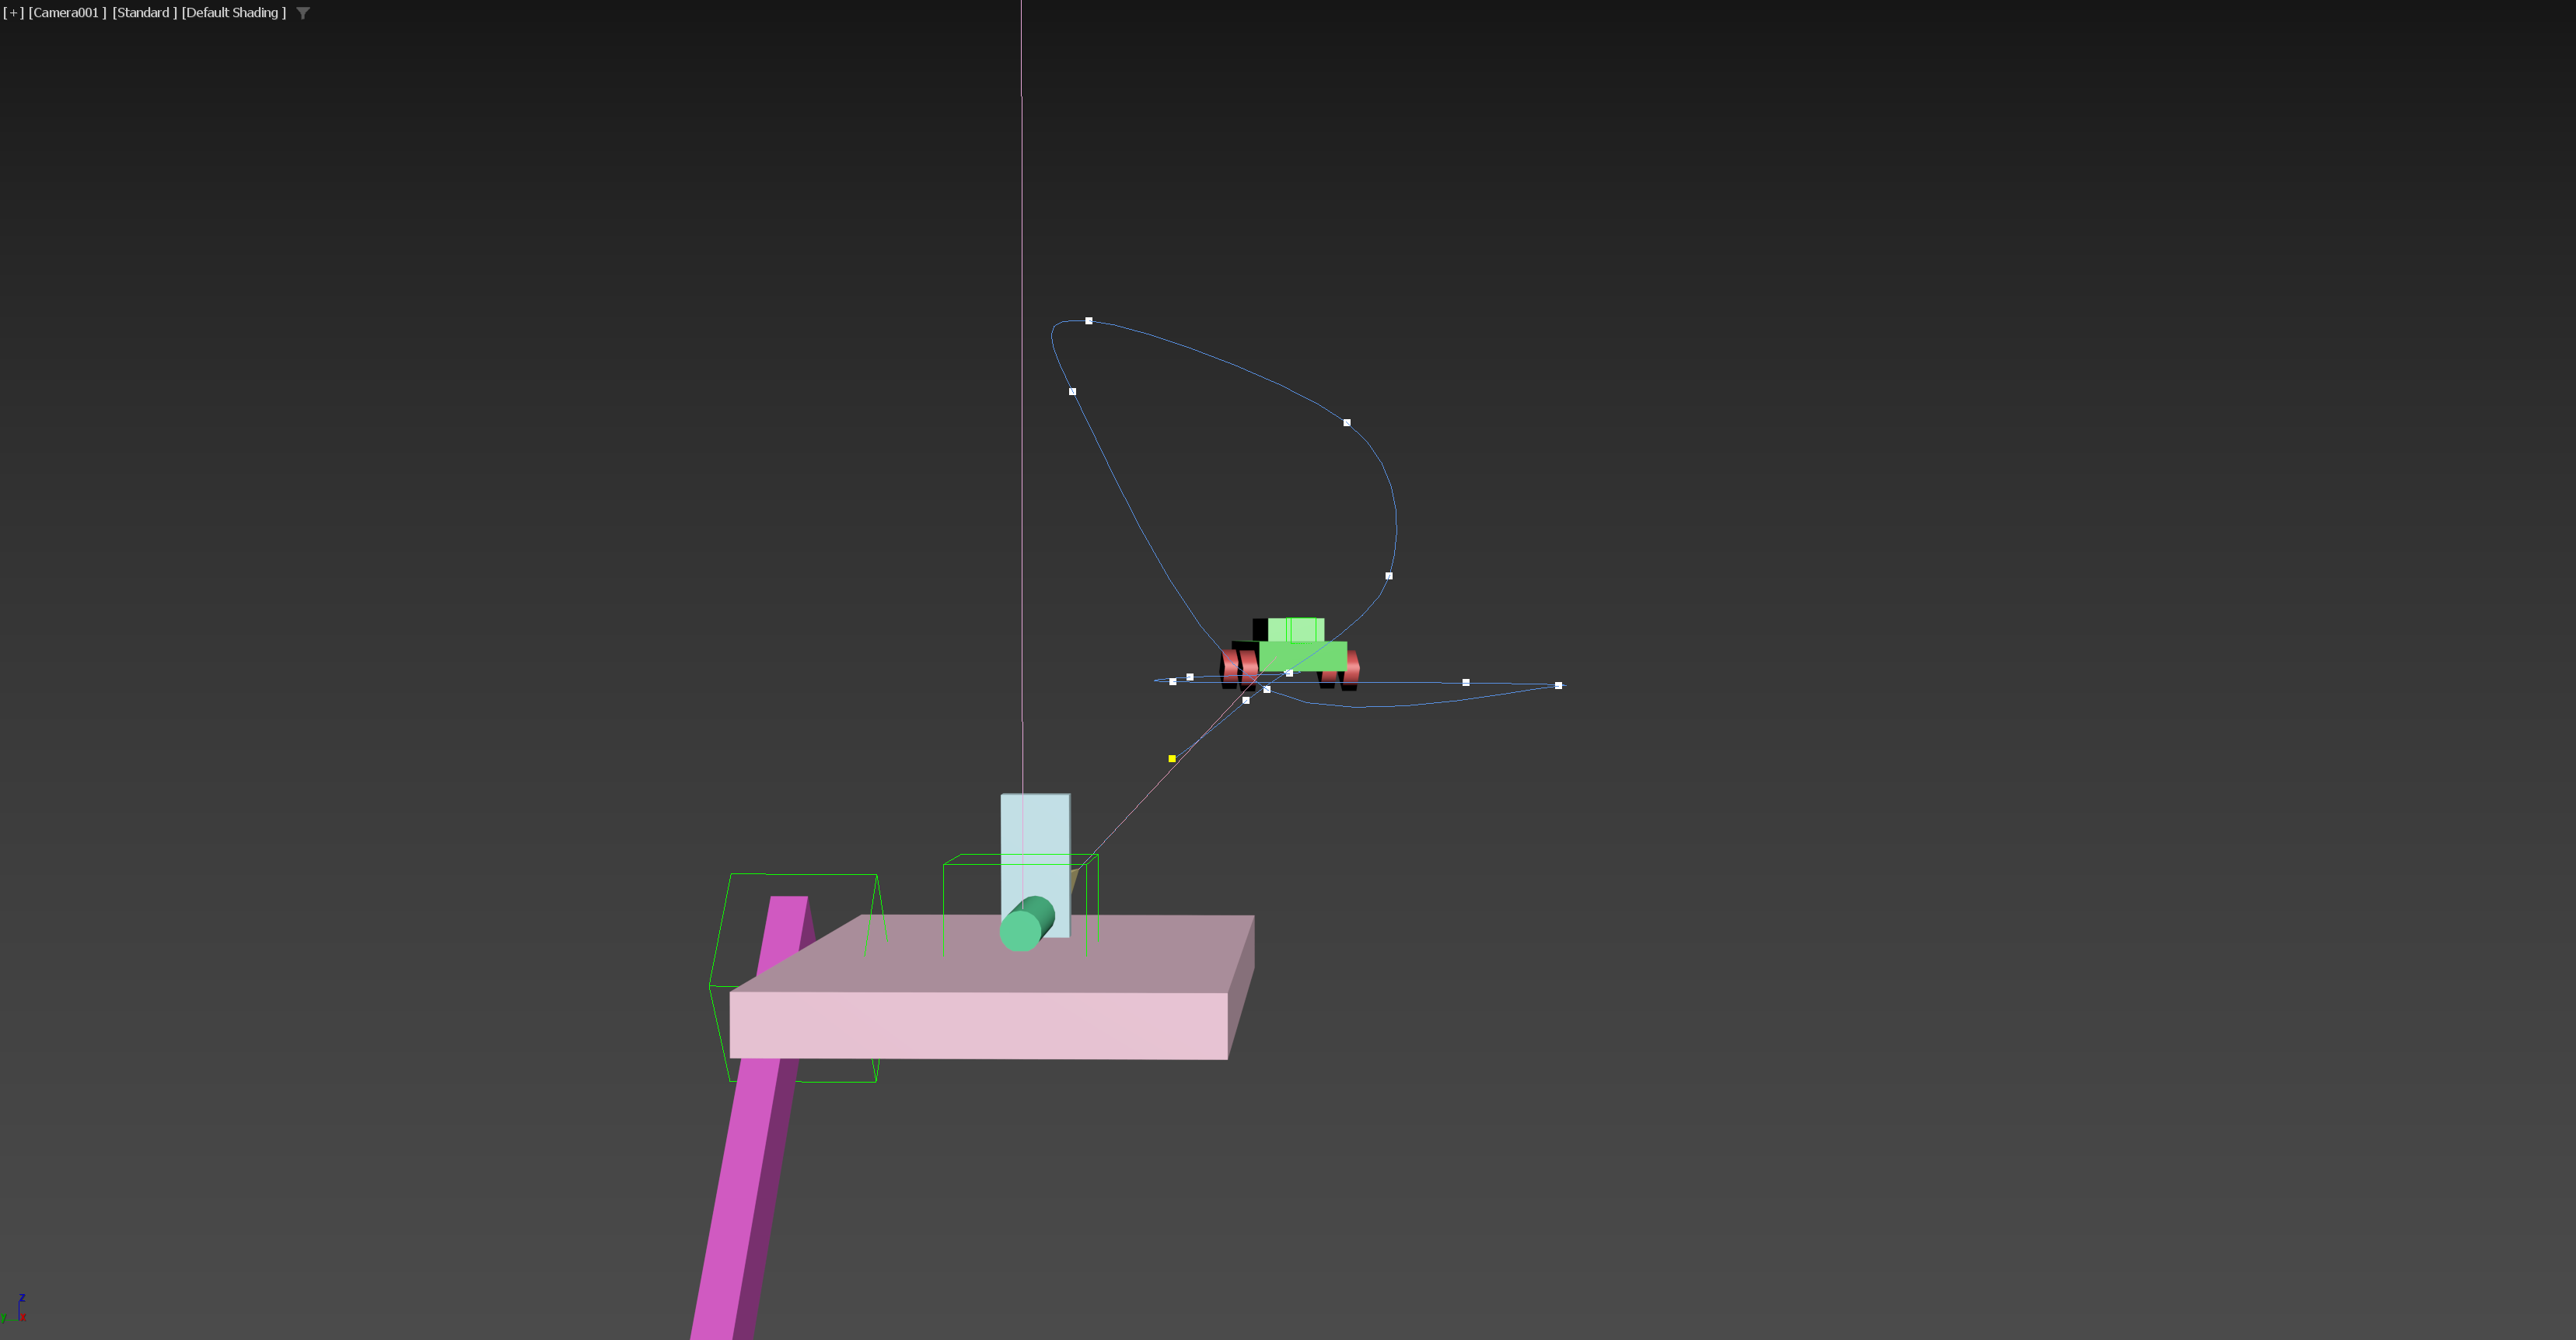
\includegraphics[width=\textwidth]{imagenes/resultado/300.png}
        \caption{Animación en el instante 300.}
    \end{subfigure}
    \caption{Animación final.}
\end{figure}